%% LyX 2.1.3 created this file.  For more info, see http://www.lyx.org/.
%% Do not edit unless you really know what you are doing.
\documentclass[english,spanish]{article}
\usepackage[T1]{fontenc}
\usepackage[utf8]{luainputenc}
\usepackage{amstext}
\usepackage{graphicx}
\usepackage{subscript}
\usepackage{babel}
\addto\shorthandsspanish{\spanishdeactivate{~<>}}

\begin{document}

\title{\textbf{Práctica 2}}


\author{Pablo Cabeza García y Diego González Domínguez}

\maketitle

\section*{Ejercicios:}
\selectlanguage{english}%
\begin{enumerate}
\item[\foreignlanguage{english}{\textbf{(a)}}] \textbf{Dado el toro de revolución usual, dibújese sobre el mismo
una geodésica cuya traza sea uno de los dos circuitos generadores.}
\end{enumerate}
\begin{center}
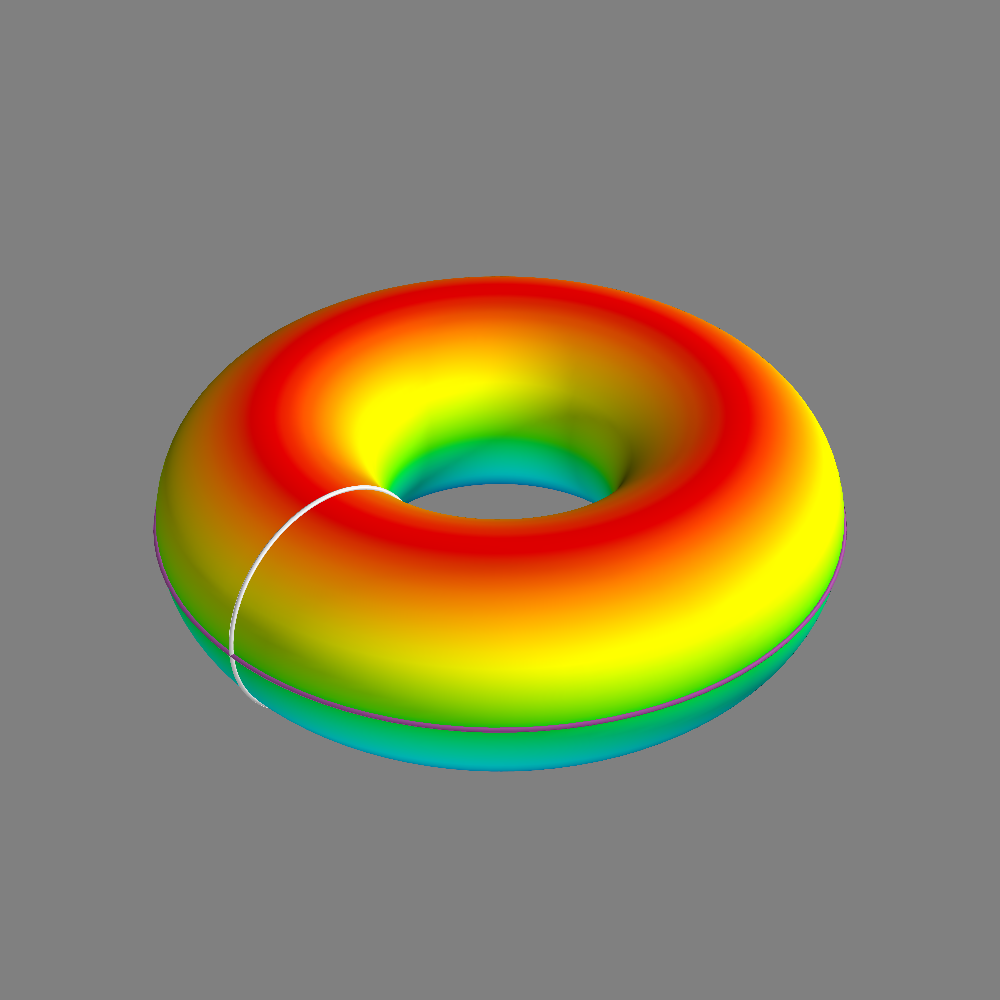
\includegraphics[scale=0.15]{img/generators}
\par\end{center}
\begin{enumerate}
\item[\foreignlanguage{english}{\textbf{(b)}}] \textbf{Dibújese sobre el toro una geodésica periódica.}
\end{enumerate}
\begin{center}
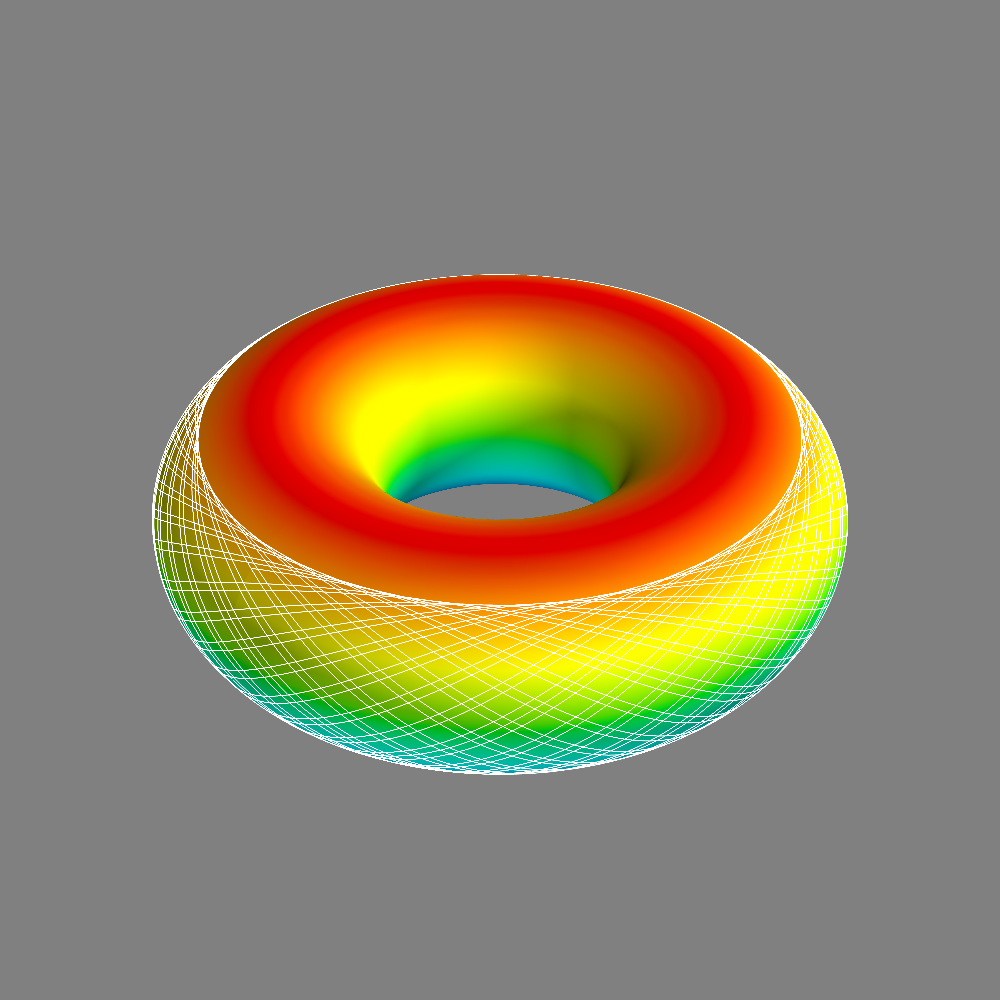
\includegraphics[scale=0.15]{img/periodic}
\par\end{center}

\begin{center}
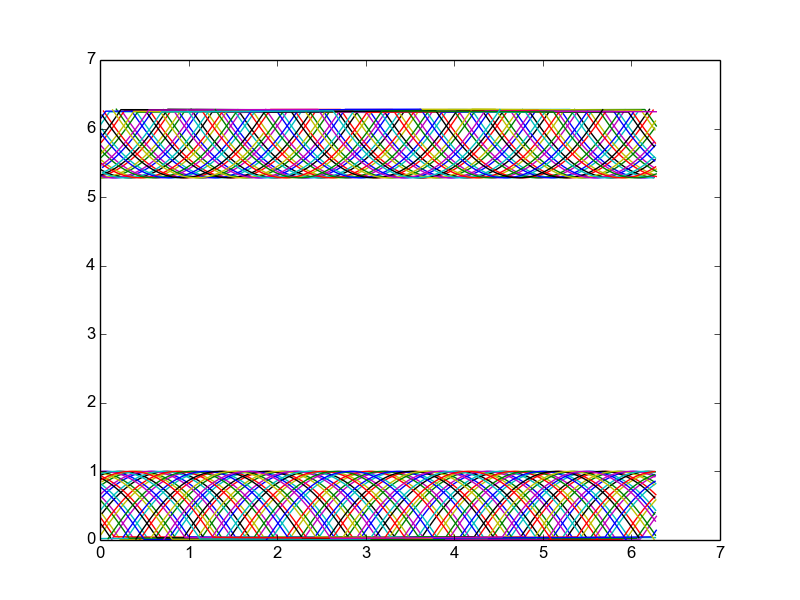
\includegraphics[scale=0.4]{img/periodic_uv}
\par\end{center}

\textbf{Dibújese sobre el toro una geodésica no periódica.}

\begin{center}
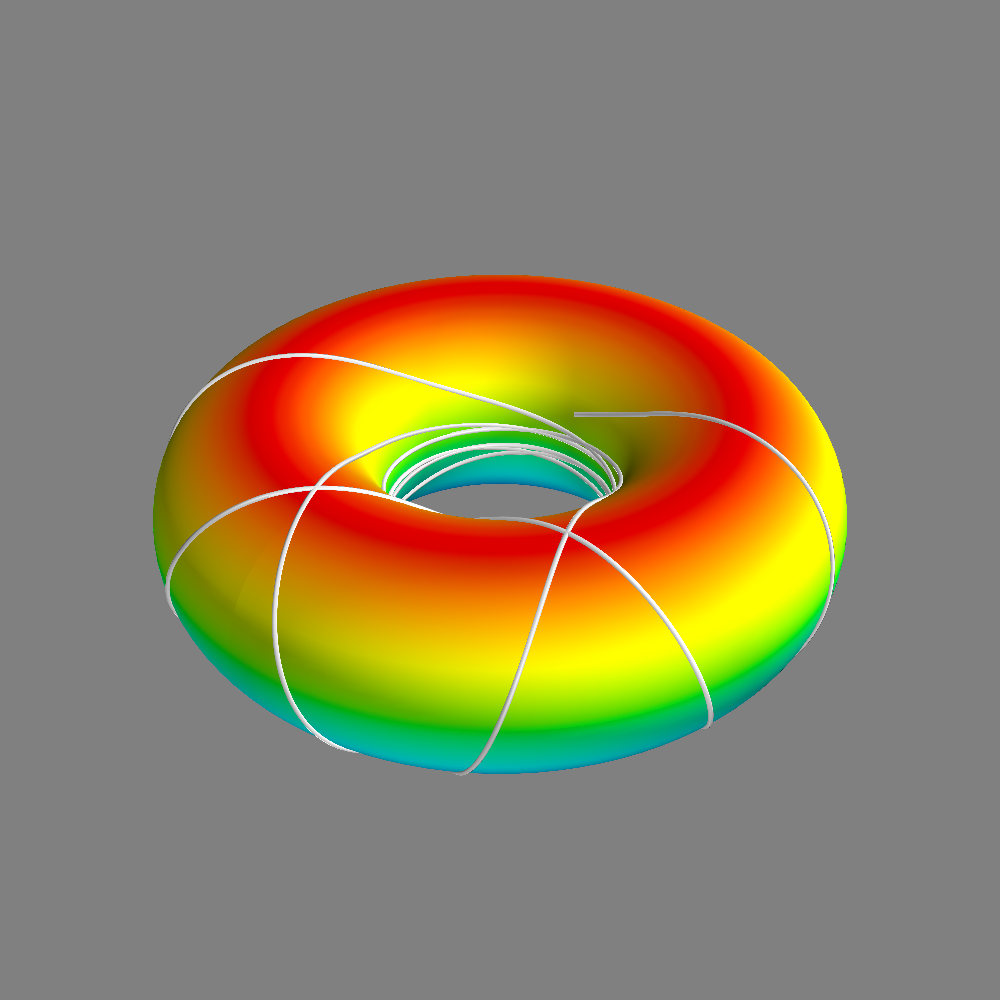
\includegraphics[scale=0.15]{img/nonperiodic}
\par\end{center}

\begin{center}
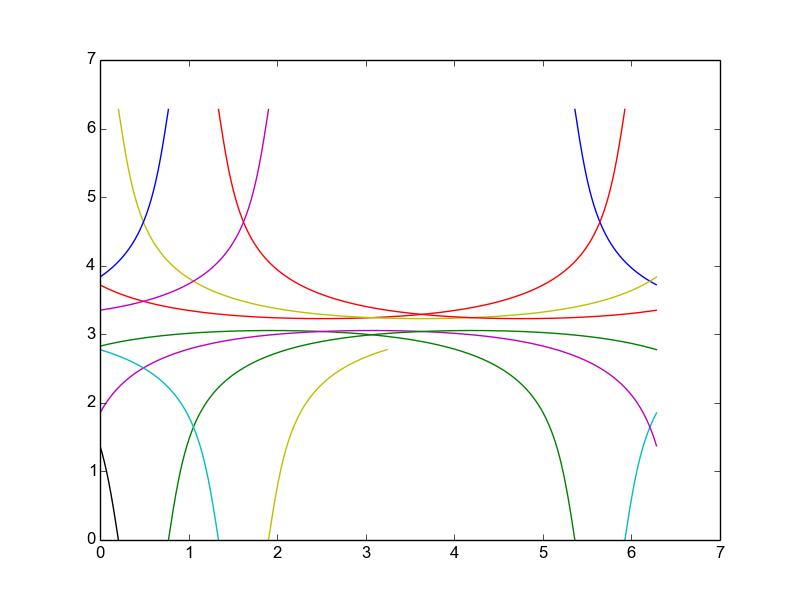
\includegraphics[scale=0.4]{img/nonperiodic_uv}
\par\end{center}
\textbf{{[}Opcional{]} ¿Sabríais obtener una geodésica que sea densa
sobre todo el toro?}

Por la parametrización de Clairaut, se obtiene que

\begin{center}
$\frac{du}{dv}=\pm\frac{r\text{·}h}{(R+r\text{·}\cos(v))\text{·}\sqrt{(R+r\text{·}\cos(v))-h^{2}}}$
\par\end{center}

donde h es el angulo entre la geodesíca y un meridiano, de manera
que según el valor de h las geodésicas pueden ser:
\selectlanguage{spanish}%
\begin{itemize}
\item h = 0: Meridianos
\item 0 < |h| < R-r: Cruzan alternativamente ambos ecuadores
\item |h| = R-r: Ecuador interior (y deogésicas asintóticas con él)
\item R-r < |h| < R+r: Cruzan el ecuador exterior
\item |h| = R+r: Ecuador exterior
\end{itemize}
.

\selectlanguage{english}%
De esta manera, para que una geodésica sea densa debe atravesar ambos
ecuadores, por lo que se tomará la segunda opción. Por ejemplo:

\begin{center}
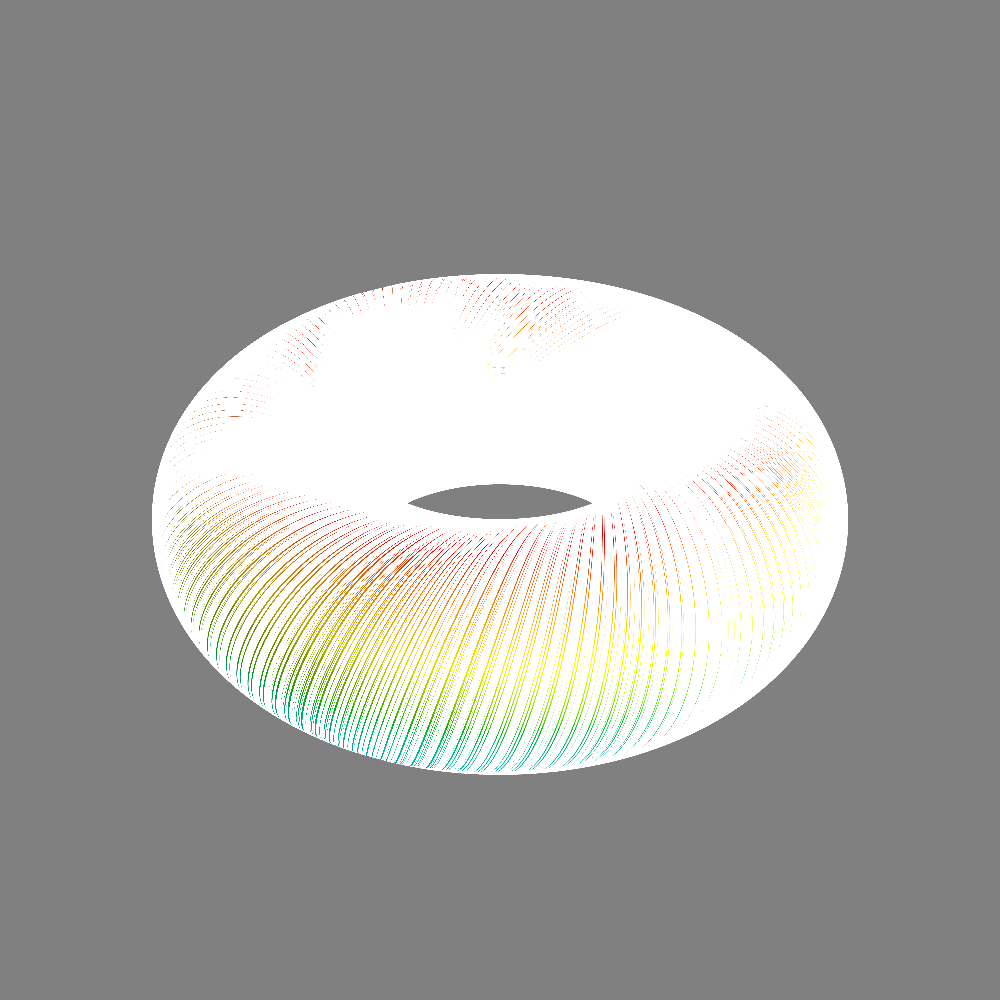
\includegraphics[scale=0.15]{img/dense}
\par\end{center}

\begin{center}
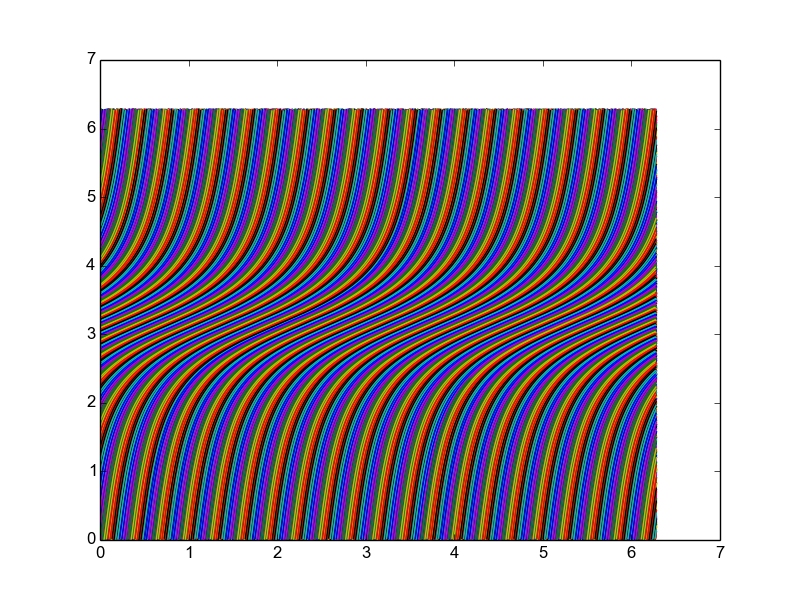
\includegraphics[scale=0.4]{img/dense_uv}
\par\end{center}
\begin{enumerate}
\item[\foreignlanguage{english}{\textbf{(c)}}] \textbf{Considérese la primera forma fundamental en el semiplano
}\textbf{\textit{v}}\textbf{ > 0 dada por }\textbf{\textit{E}}\textbf{
= G = 1/}\textbf{\textit{v}}\textbf{\textsuperscript{\textbf{2}}
y }\textbf{\textit{F}}\textbf{ = 0. Dibújese sus geodésicas.}
\end{enumerate}
\begin{center}
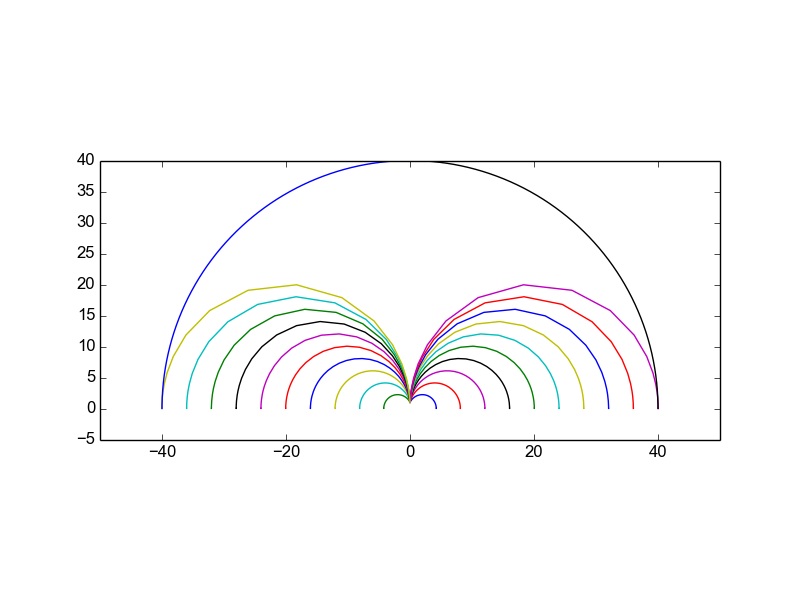
\includegraphics[scale=0.4]{img/poincare}
\par\end{center}

\textbf{{[}Opcional{]} ¿Sabríais encontrar expresiones analíticas
de las mismas?}

\selectlanguage{spanish}%
A aprtir de la primera forma fundamental del semiplano de Poincaré:

\begin{center}
$dC^{2}(u,v)=\frac{du^{2}+dv^{2}}{v^{2}}$
\par\end{center}

Para obtener la ``recta'' entre dos puntos con la menor energía:

\begin{center}
$\varepsilon=\intop dC^{2}dt=\intop\sqrt{\frac{1+w^{2}}{v^{2}}}du=\intop L(v,w)\thinspace du$
, con $w=\frac{dv}{du}$
\par\end{center}

Escribiendo las ecuaciones para minimizar la distancia:

\begin{center}
$\frac{d}{du}\frac{\partial L}{\partial w}-\frac{\partial L}{\partial v}=0\qquad\rightarrow\qquad v\frac{d^{2}v}{du^{2}}+\left(1+\left(\frac{dv}{du}\right)^{2}\right)=0$
\par\end{center}

que sería la ecuación de la geodésica \textit{v}(\textit{u}), aunque
sería muy difícil de resolver.

Para simplificarlas, y dada la forma de las geodésicas que hemos obtenido
en el aprtado anterior, se usa la ecuación para una circunferencia
de readio R y centro (\textit{u}\textsubscript{0},\textit{v}\textsubscript{0}):

\begin{center}
$(u-u_{0})^{2}+(v-v_{0})^{2}=R^{2}$
\par\end{center}

Sustituyendo en la ecuación de las geodésicas vemos que es solución
si \textit{v}\textsubscript{0} = 0, en cuyo caso las geodésicas son
semicirculos de readio R y centro (\textit{u}\textsubscript{0},0):

\begin{center}
$v(u)=\sqrt{R^{2}-(u-u_{0})^{2}}$
\par\end{center}
\end{document}
